Lampiran berisi dokumen pendukung dan tangkapan layar yang menunjang pembahasan proyek akhir.

\setcounter{figure}{0}
\renewcommand{\thefigure}{L.\arabic{figure}}
\captionsetup{hypcap=false}

\section*{Rekapitulasi Kuesioner InternSync}
\addcontentsline{toc}{section}{Rekapitulasi Kuesioner InternSync}

{\small
\noindent\textbf{Link Responden Siswa:}\par
\noindent\href{https://docs.google.com/forms/d/e/1FAIpQLSf-MIfhVixnjja9oZIZ9ugWZsfemnbiRVDqD0d2gpPSG5jwow/viewform}{\texttt{https://docs.google.com/forms/d/e/1FAIpQLSf-MIfhVixnjja9oZIZ9ugW}\\\texttt{ZsfemnbiRVDqD0d2gpPSG5jwow/viewform}}\par
\noindent\textbf{Link Responden Guru:}\par
\noindent\href{https://docs.google.com/forms/d/e/1FAIpQLSduP57CQ_8BKu3W4xbrgNGjhA2UW4OOY5X_p_qyXWZXBjylFQ/viewform}{\texttt{https://docs.google.com/forms/d/e/1FAIpQLSduP57CQ\_8BKu3W4xbrgNGjh}\\\texttt{A2UW4OOY5X\_p\_qyXWZXBjylFQ/viewform}}\par
}
\newgeometry{left=1.5cm,right=1.5cm,top=1.5cm,bottom=3cm}

\begin{center}
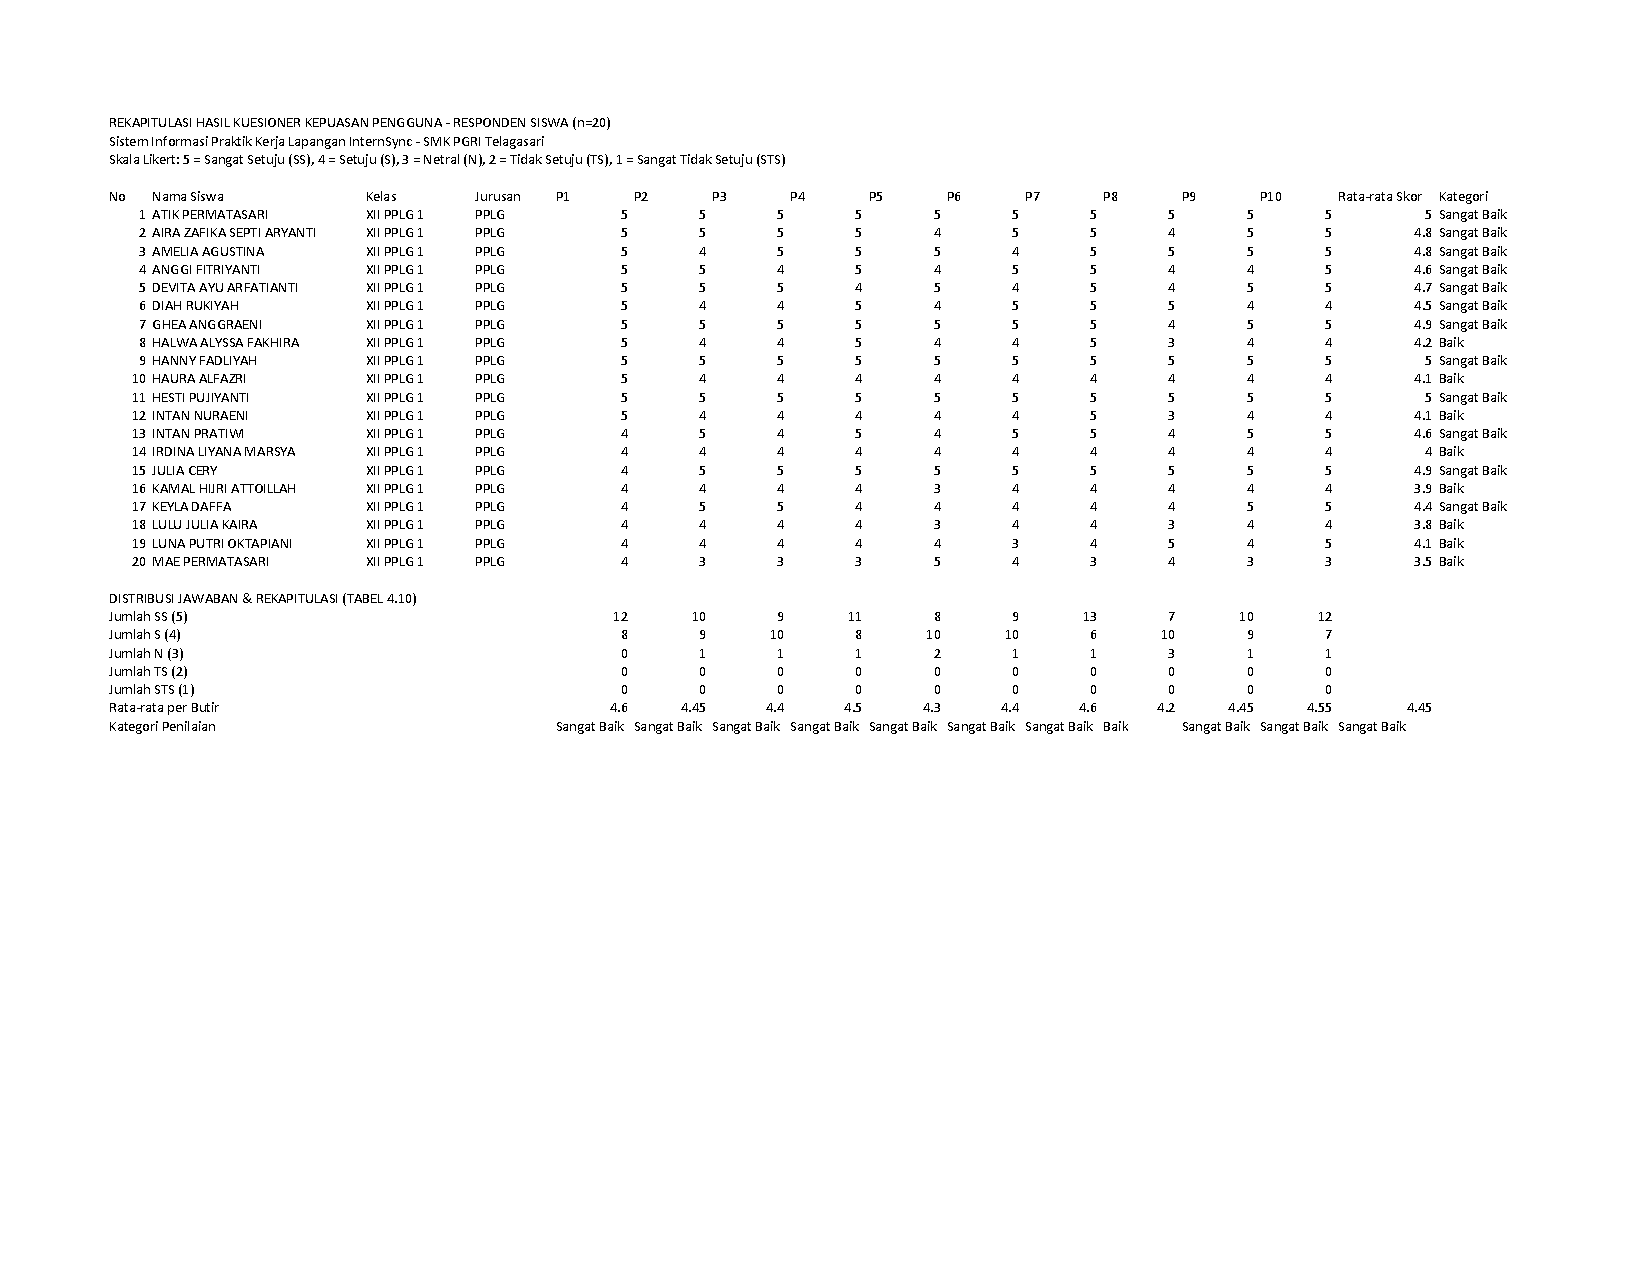
\includegraphics[page=1,angle=90,width=0.96\textheight,height=0.96\textwidth,keepaspectratio,frame]{lampiran/Rekapitulasi_Kuesioner_InternSync.pdf}
\captionof{figure}{Rekapitulasi Kuesioner InternSync (Halaman 1)}\label{fig:lampiran-kuesioner-1}
\end{center}
\clearpage

\begin{center}
\includegraphics[page=2,angle=90,width=0.96\textheight,height=0.96\textwidth,keepaspectratio,frame]{lampiran/Rekapitulasi_Kuesioner_InternSync.pdf}
\captionof{figure}{Rekapitulasi Kuesioner InternSync (Halaman 2)}\label{fig:lampiran-kuesioner-2}
\end{center}
\clearpage

\begin{center}
\adjustbox{angle=90,width=0.96\textheight,height=0.96\textwidth,keepaspectratio,frame}{%
\begin{tikzpicture}[x=1bp,y=1bp]
\path[use as bounding box] (0,0) rectangle (792,612);
\node[anchor=south west,inner sep=0pt] at (0,0)
  {\includegraphics[page=3,width=792bp,height=612bp,keepaspectratio]{lampiran/Rekapitulasi_Kuesioner_InternSync.pdf}};
\fill[white] (49,530) rectangle (350,548);
\node[anchor=west,inner sep=0pt,font=\sffamily\fontsize{8.18bp}{9bp}\selectfont] at (52.44,539.04)
  {Berdasarkan Laporan Subbab 4.9 (Tabel 4.12) \& Subbab 4.8 (Kuesioner Kepuasan)};
\end{tikzpicture}}
\captionof{figure}{Rekapitulasi Kuesioner InternSync (Halaman 3)}\label{fig:lampiran-kuesioner-3}
\end{center}
\clearpage

\begin{center}
\includegraphics[page=4,angle=90,width=0.96\textheight,height=0.96\textwidth,keepaspectratio,frame]{lampiran/Rekapitulasi_Kuesioner_InternSync.pdf}
\captionof{figure}{Rekapitulasi Kuesioner InternSync (Halaman 4)}\label{fig:lampiran-kuesioner-4}
\end{center}
\clearpage

\restoregeometry
\clearpage

\section*{Dokumen PDF Pendukung}
\addcontentsline{toc}{section}{Dokumen PDF Pendukung}

\begin{center}
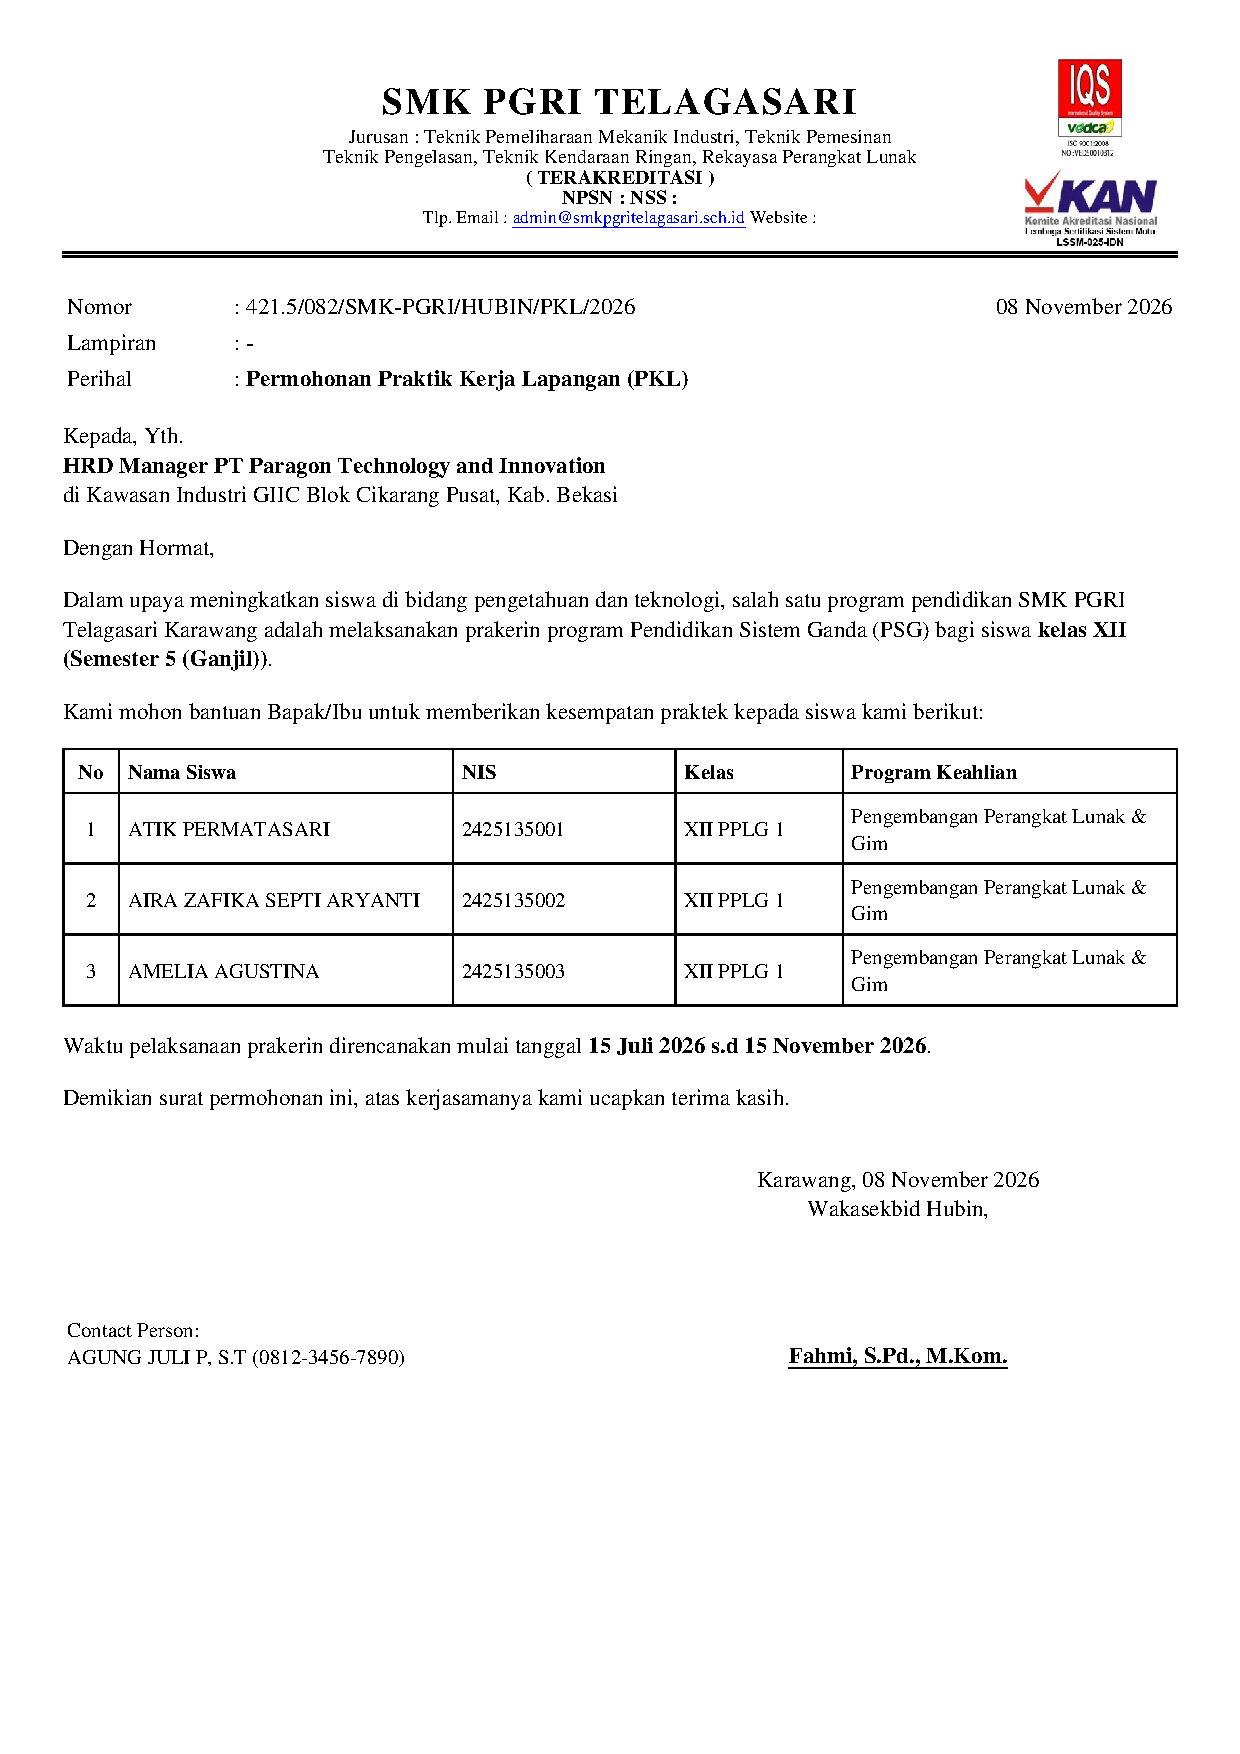
\includegraphics[page=1,width=0.90\textwidth,height=0.72\textheight,keepaspectratio,frame]{lampiran/1_Surat_Pengajuan_PKL.pdf}
\captionof{figure}{Surat Pengajuan PKL}\label{fig:lampiran-01}
\end{center}
\clearpage

\begin{center}
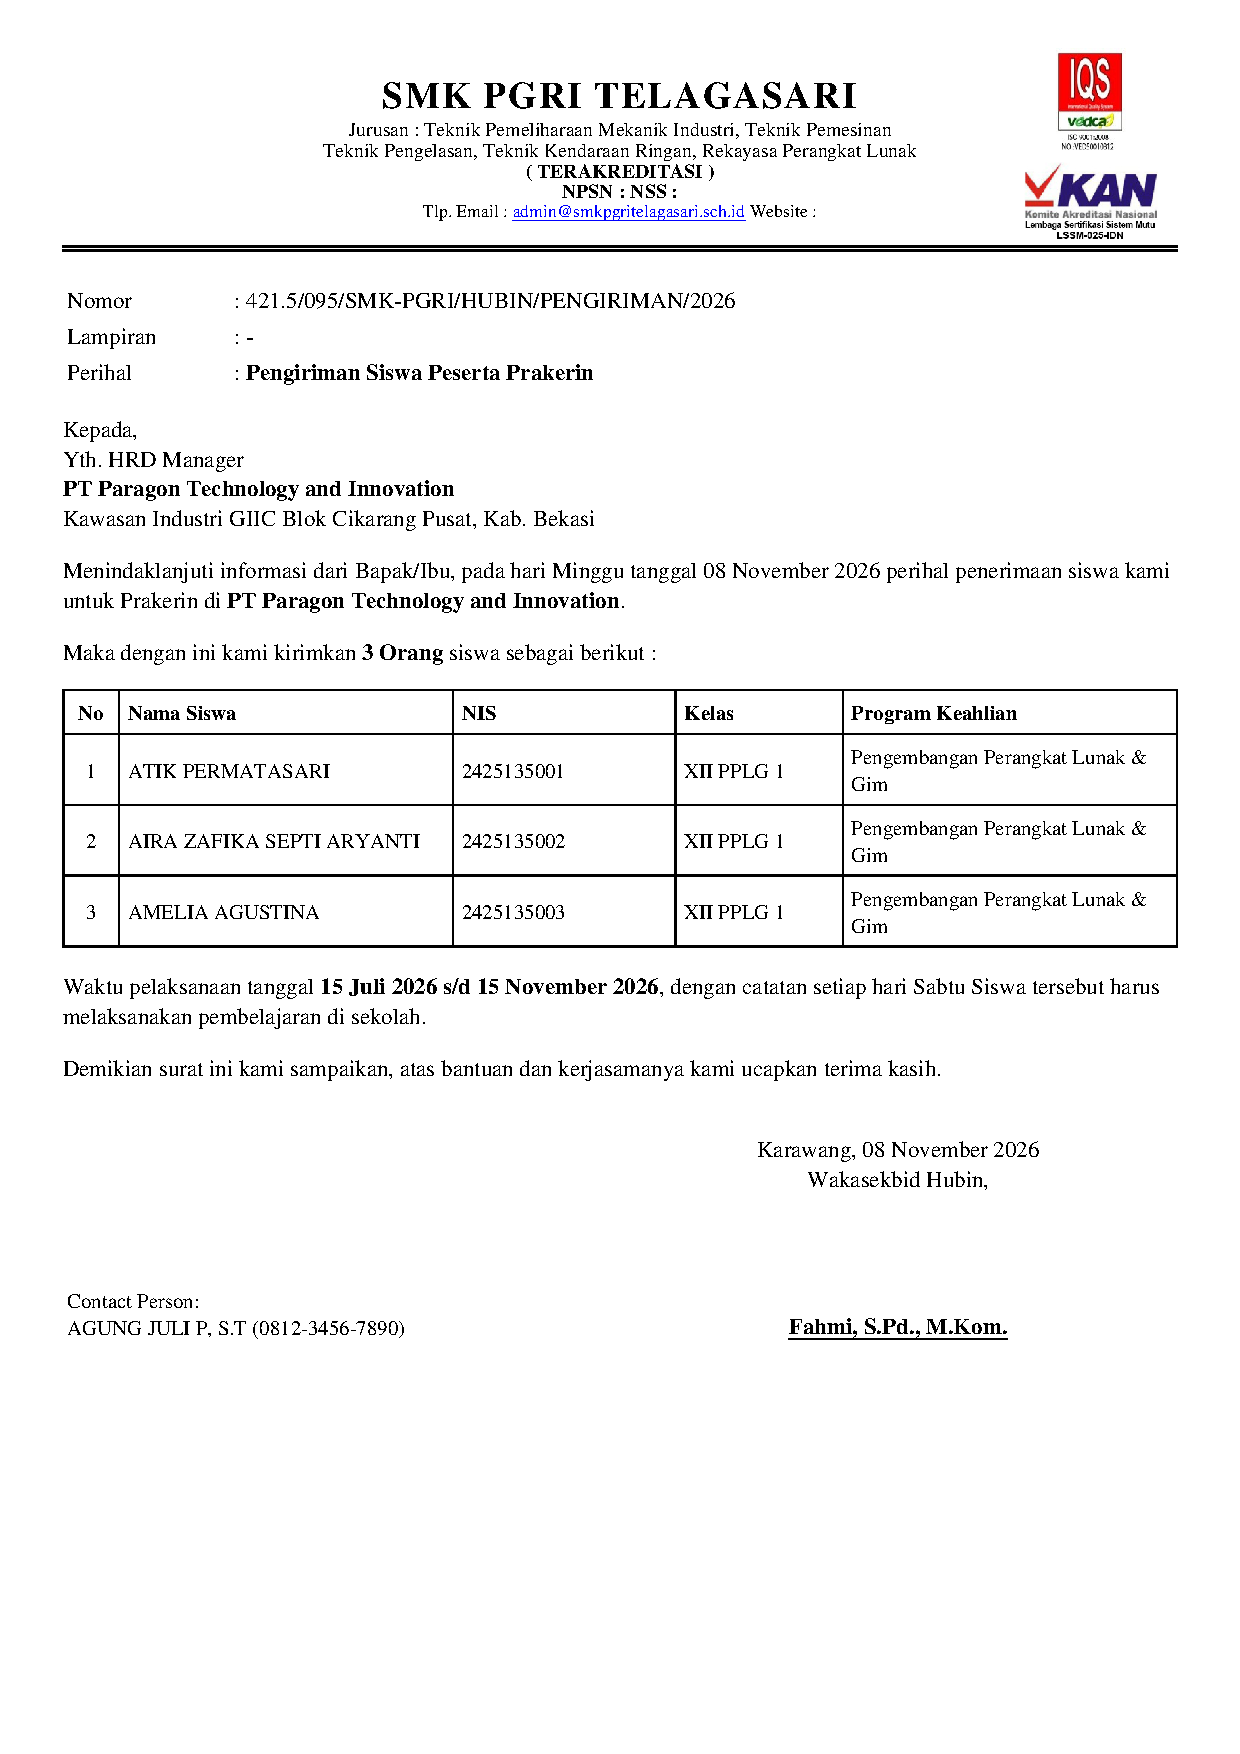
\includegraphics[page=1,width=0.90\textwidth,height=0.72\textheight,keepaspectratio,frame]{lampiran/2_Surat_Pengiriman_Siswa.pdf}
\captionof{figure}{Surat Pengiriman Siswa PKL}\label{fig:lampiran-02}
\end{center}
\clearpage

\begin{center}
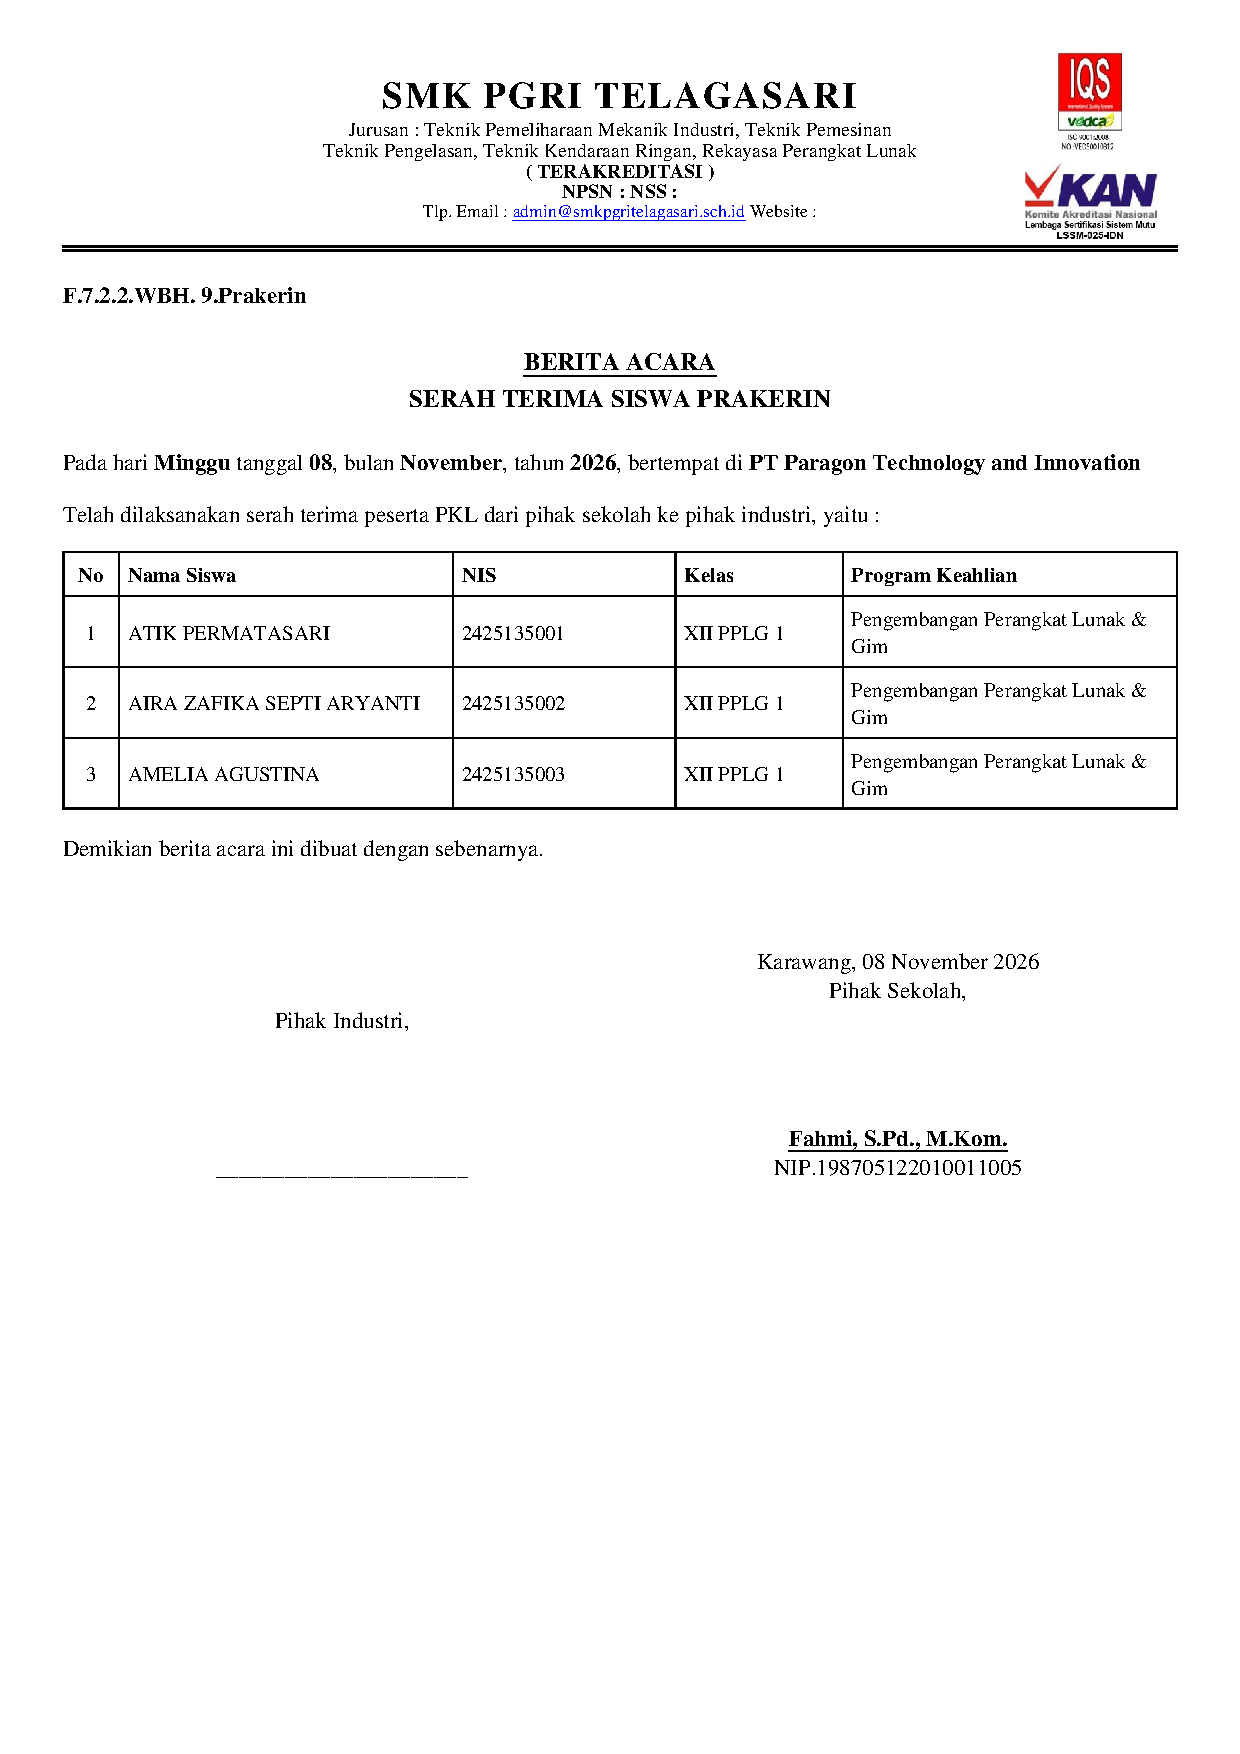
\includegraphics[page=1,width=0.90\textwidth,height=0.72\textheight,keepaspectratio,frame]{lampiran/3_Berita_Acara_Serah_Terima.pdf}
\captionof{figure}{Berita Acara Serah Terima Siswa PKL}\label{fig:lampiran-03}
\end{center}
\clearpage

\begin{center}
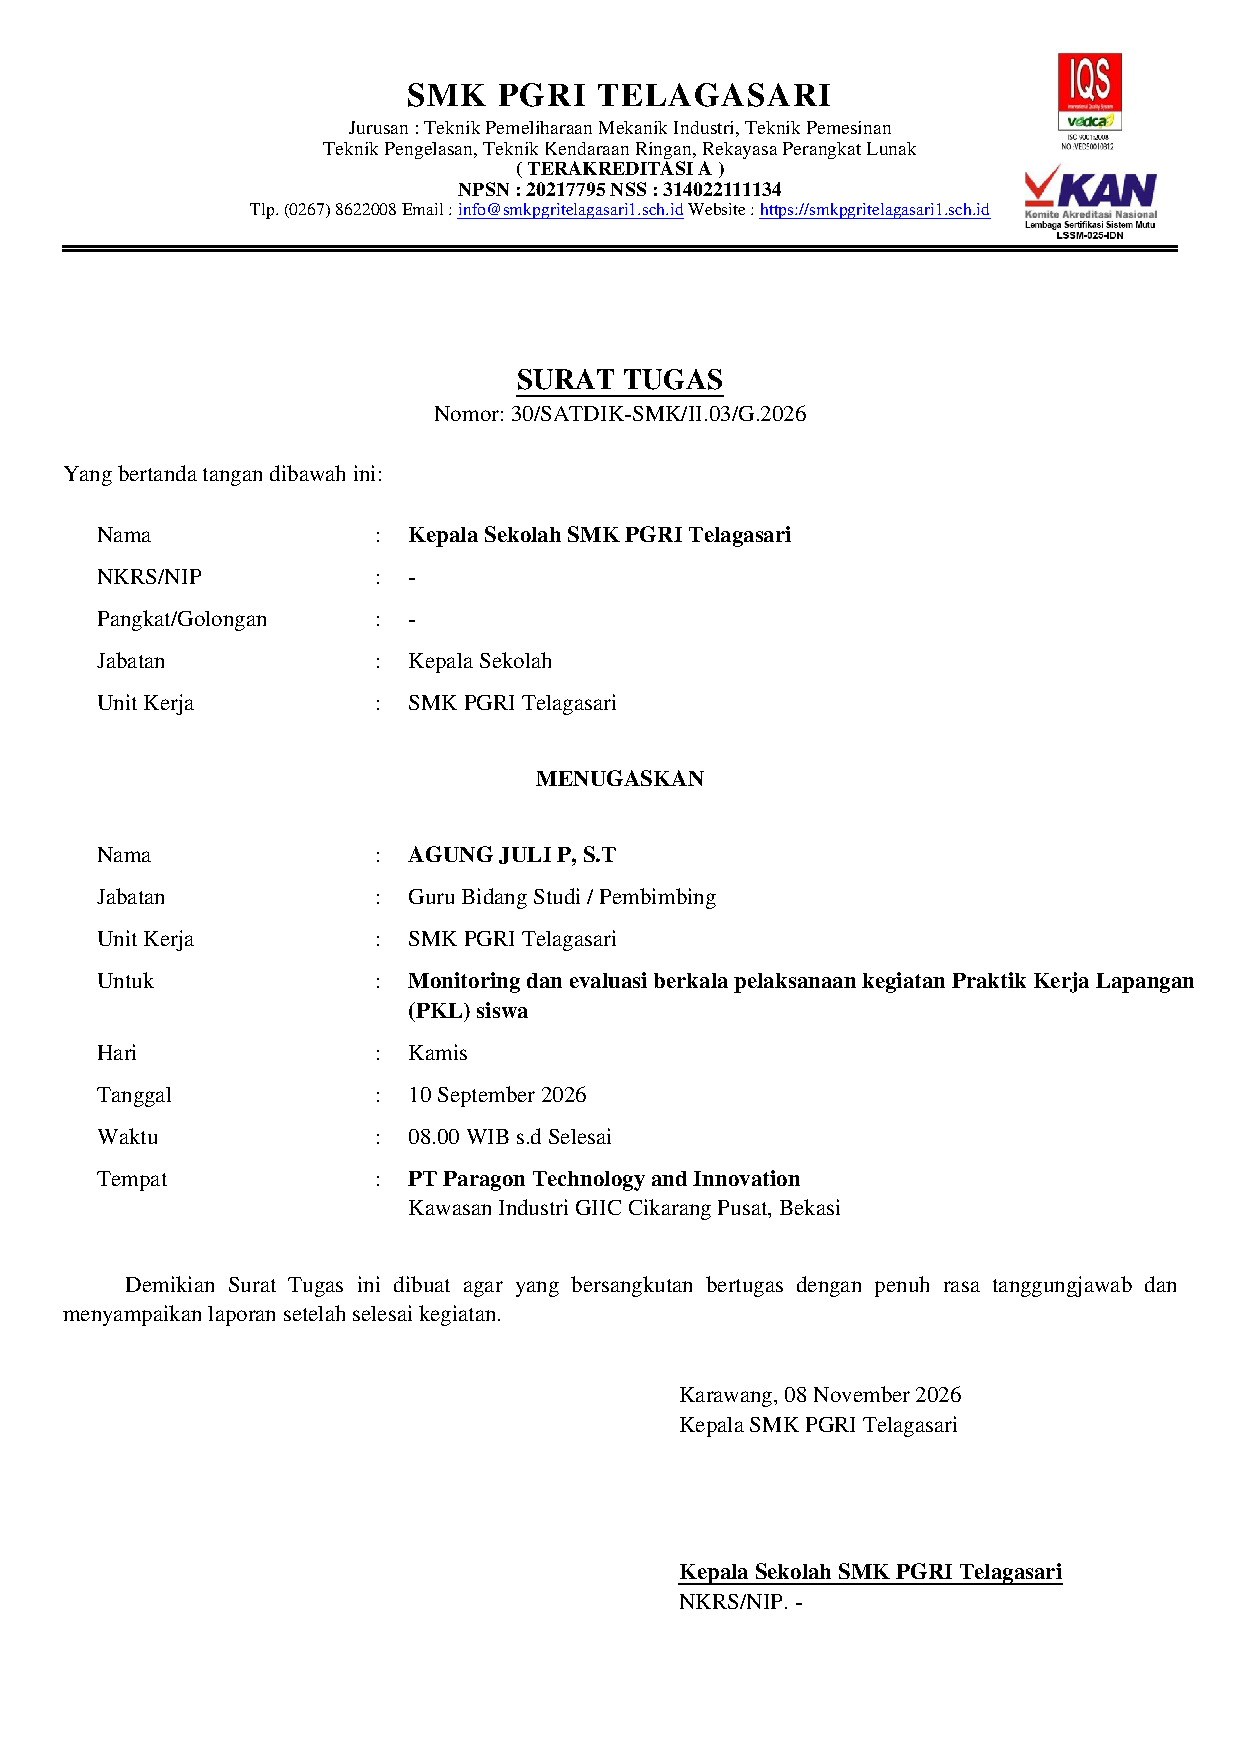
\includegraphics[page=1,width=0.90\textwidth,height=0.72\textheight,keepaspectratio,frame]{lampiran/4_SPPD_Kunjungan_Industri.pdf}
\captionof{figure}{Surat Perintah Perjalanan Dinas Kunjungan Industri}\label{fig:lampiran-04}
\end{center}
\clearpage

\begin{center}
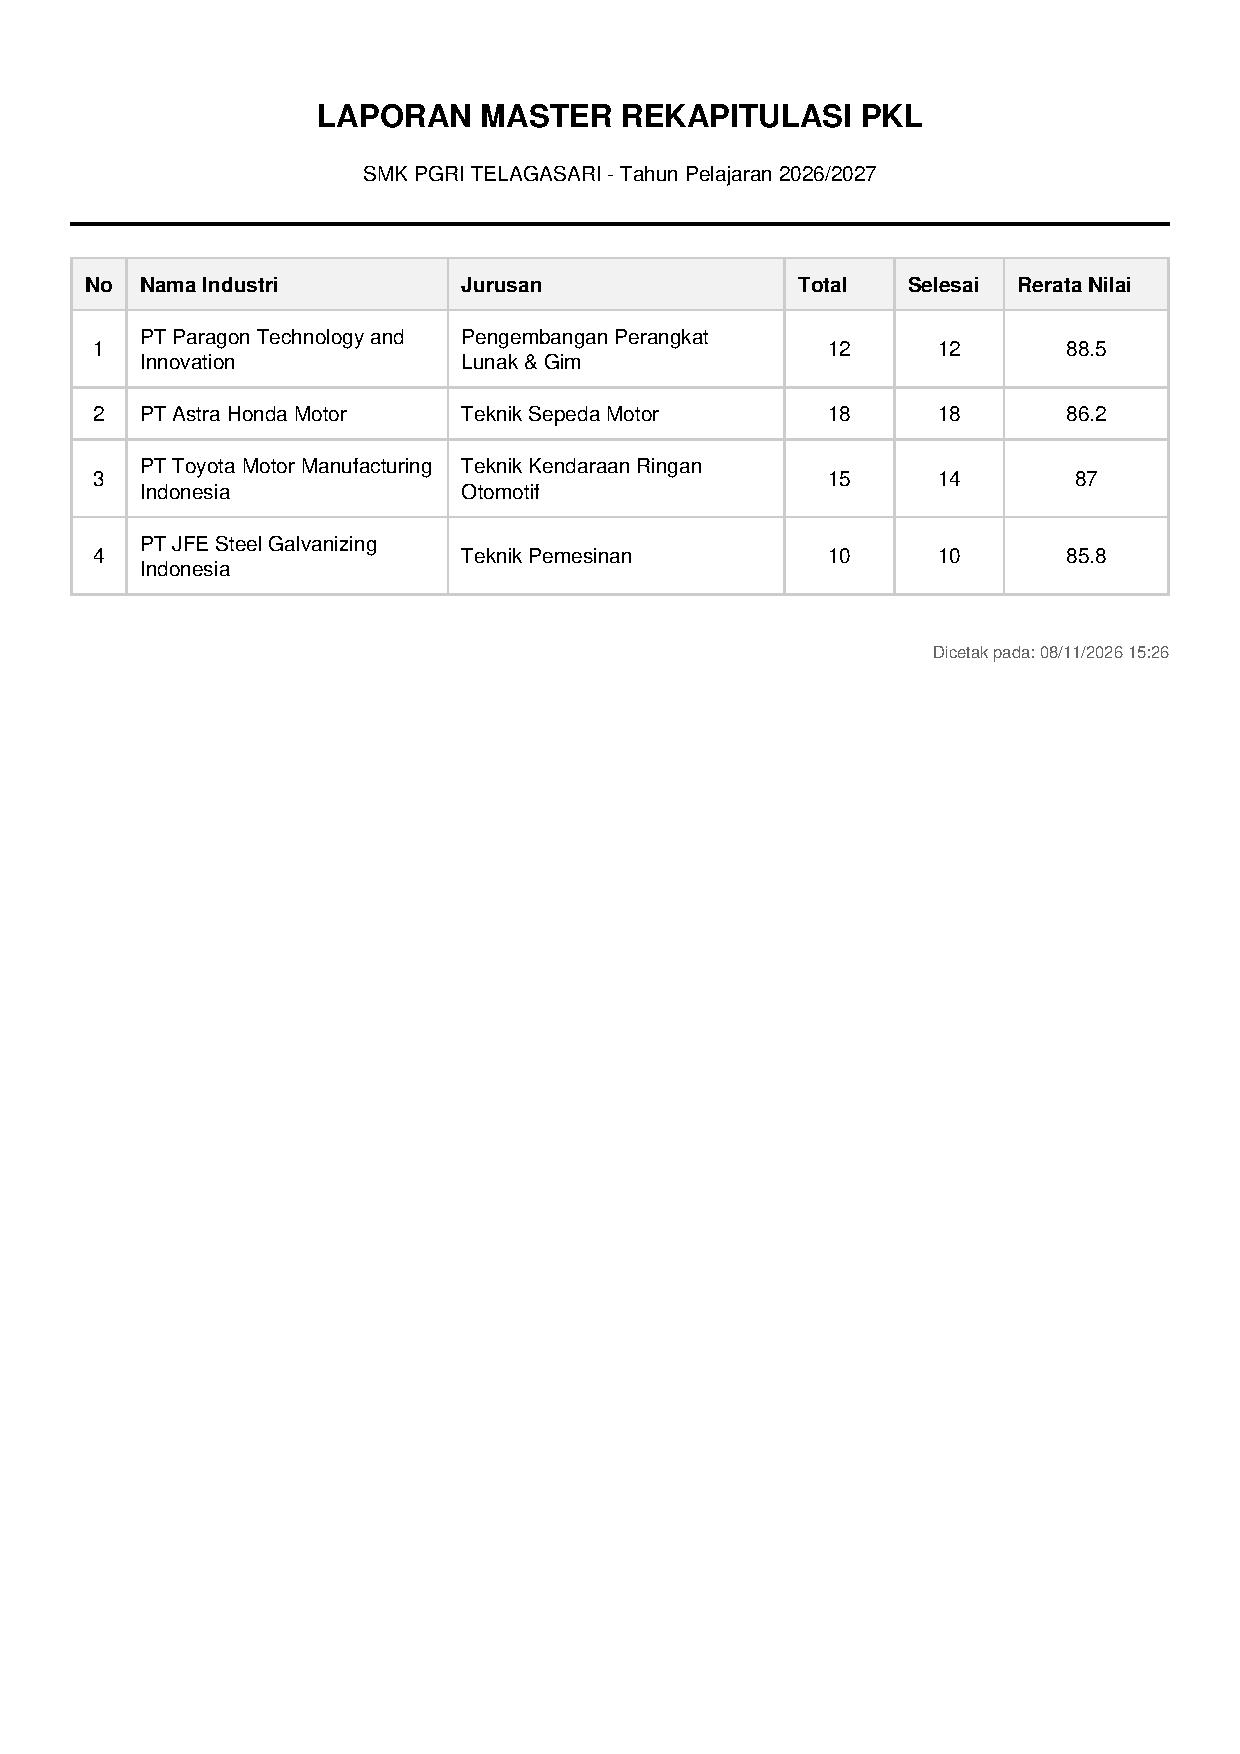
\includegraphics[page=1,width=0.90\textwidth,height=0.72\textheight,keepaspectratio,frame]{lampiran/5_Laporan_Master_Rekap_PKL.pdf}
\captionof{figure}{Laporan Master Rekapitulasi PKL}\label{fig:lampiran-05}
\end{center}
\clearpage

\begin{center}
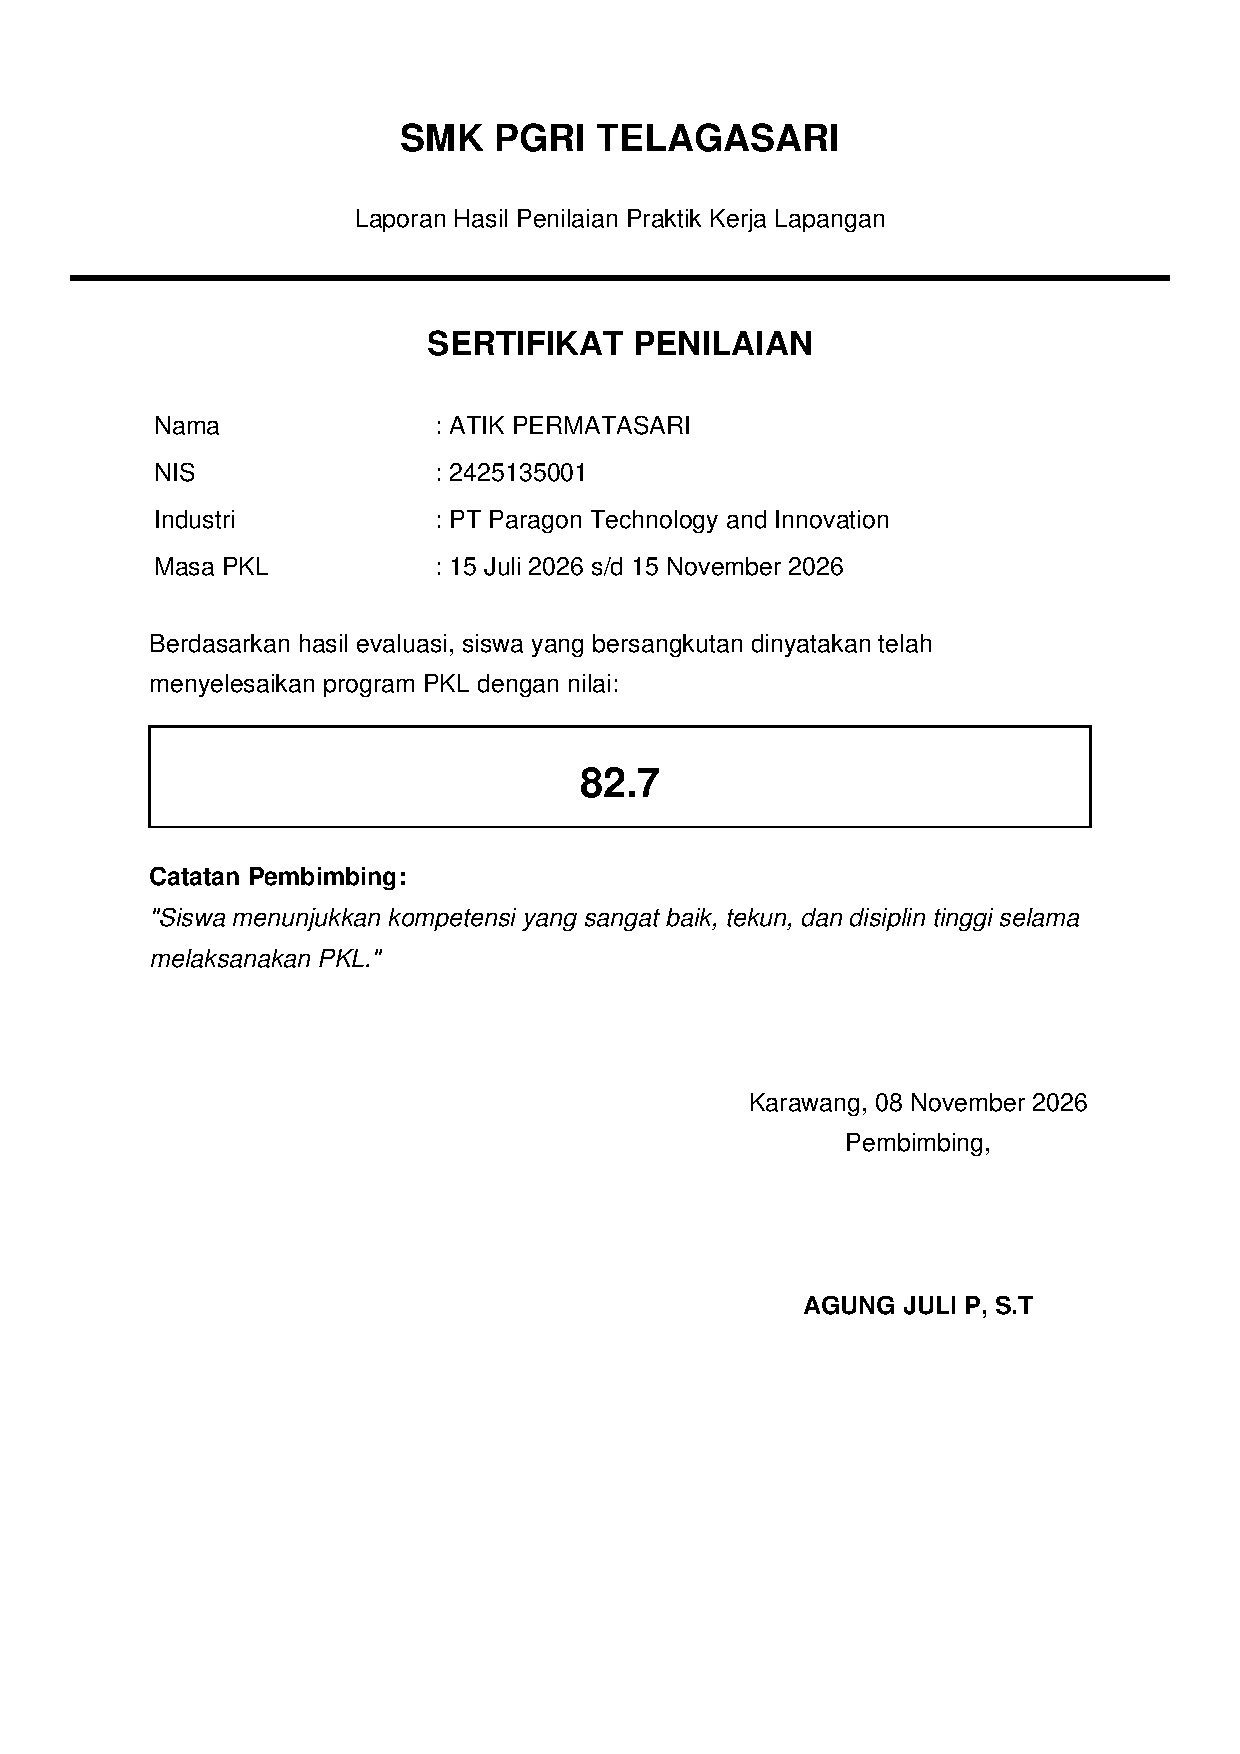
\includegraphics[page=1,width=0.90\textwidth,height=0.72\textheight,keepaspectratio,frame]{lampiran/8_Rapor_Nilai_PKL_Siswa.pdf}
\captionof{figure}{Rapor Nilai PKL Siswa}\label{fig:lampiran-06}
\end{center}
\clearpage

\begin{center}
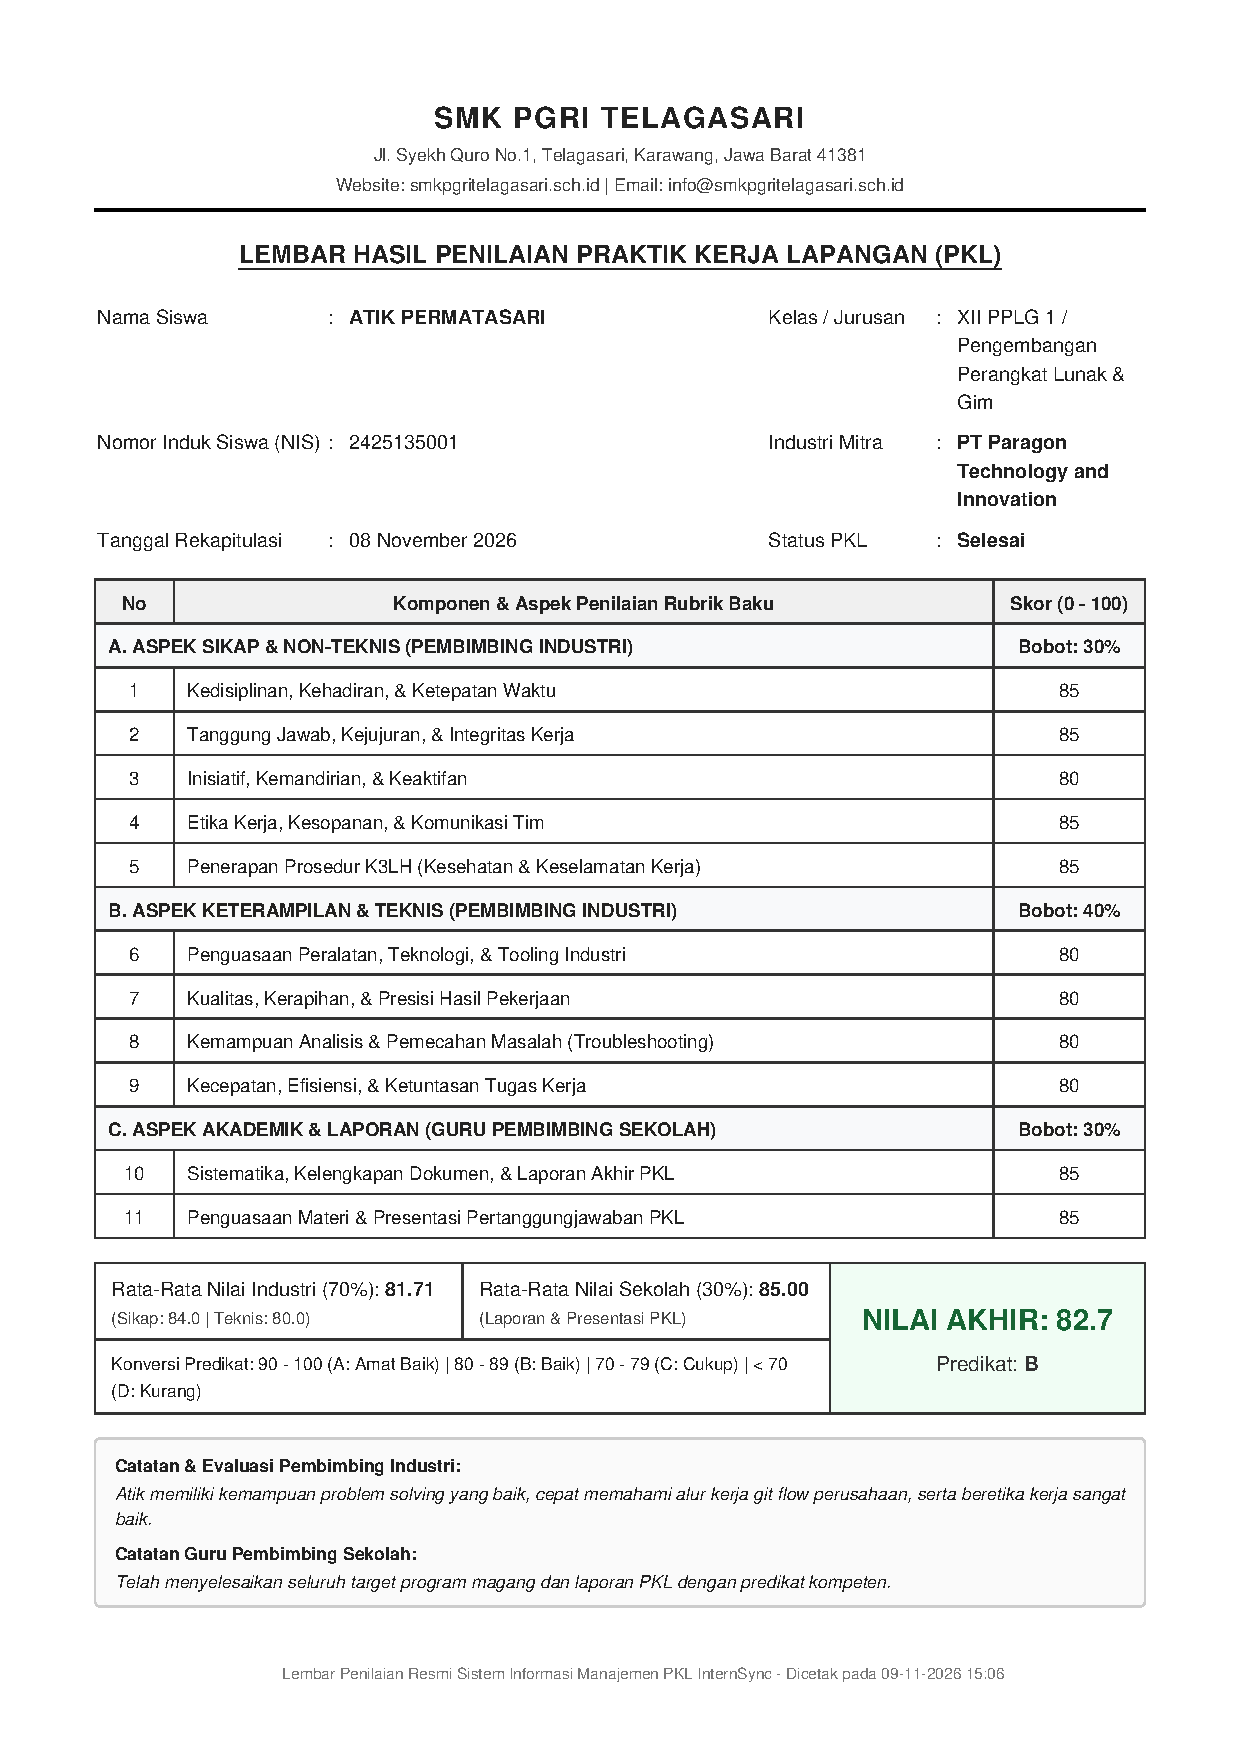
\includegraphics[page=1,width=0.90\textwidth,height=0.72\textheight,keepaspectratio,frame]{lampiran/9_Lembar_Penilaian_PKL_Siswa.pdf}
\captionof{figure}{Lembar Penilaian PKL Siswa}\label{fig:lampiran-07}
\end{center}
\clearpage

\begin{center}
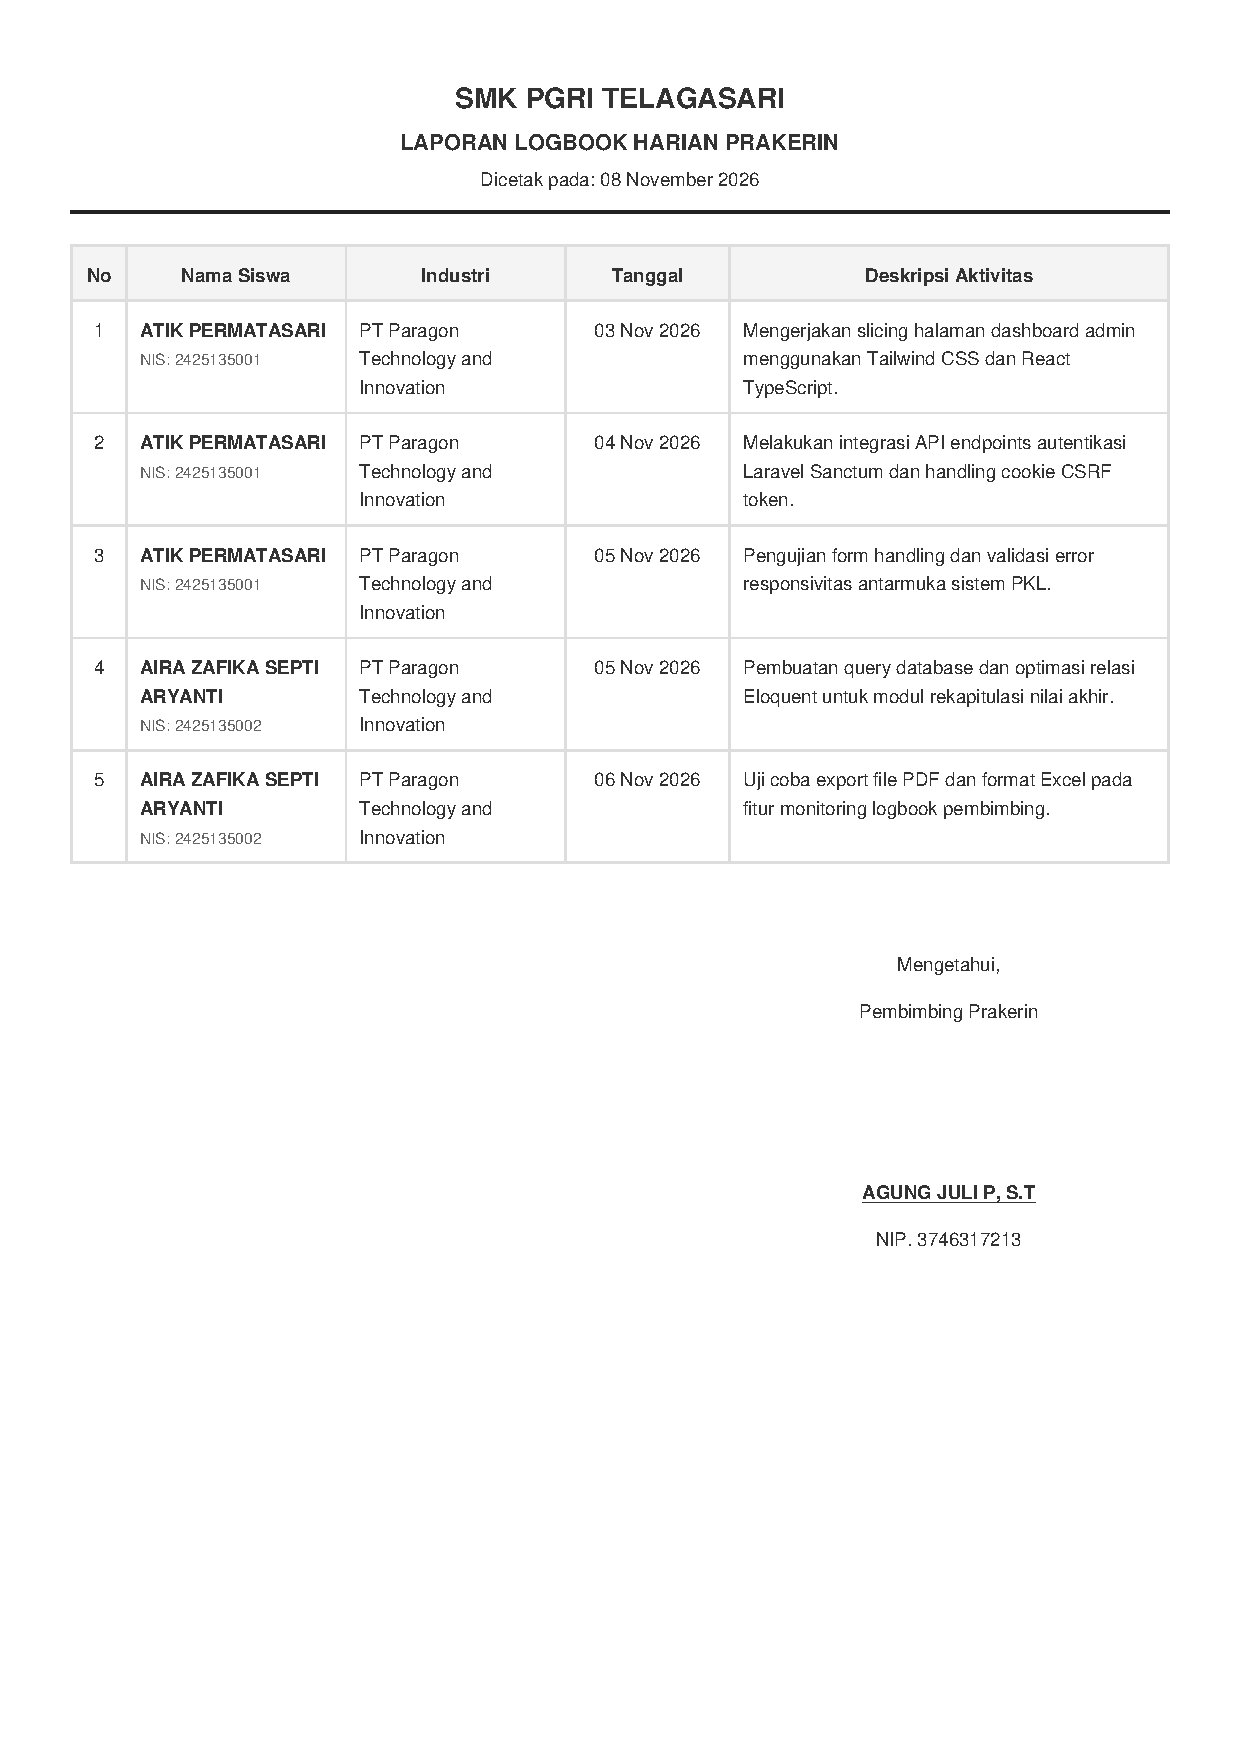
\includegraphics[page=1,width=0.90\textwidth,height=0.72\textheight,keepaspectratio,frame]{lampiran/10_Laporan_Rekap_Logbook_Siswa.pdf}
\captionof{figure}{Laporan Rekapitulasi Logbook Siswa}\label{fig:lampiran-08}
\end{center}
\clearpage

\section*{Tangkapan Layar Rekapitulasi dan Laporan}
\addcontentsline{toc}{section}{Tangkapan Layar Rekapitulasi dan Laporan}

\begin{center}
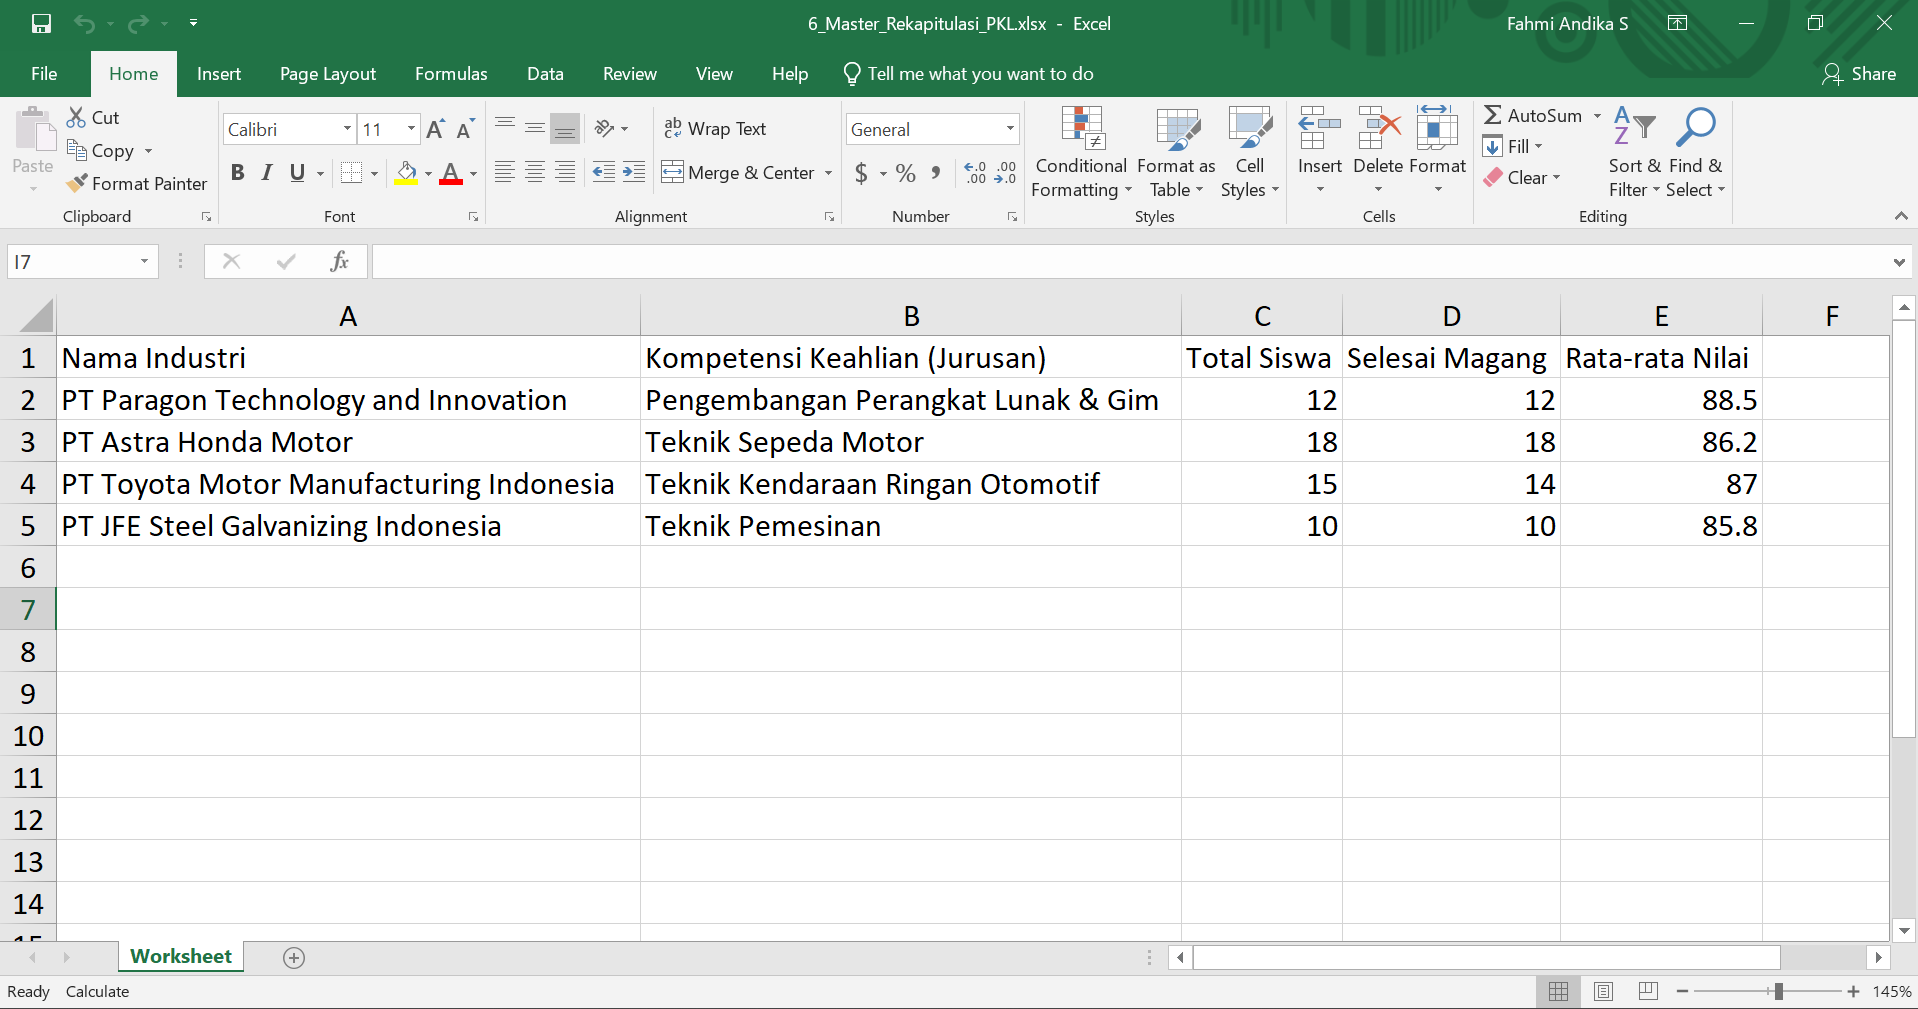
\includegraphics[width=0.94\textwidth,height=0.36\textheight,keepaspectratio]{lampiran/6_Master_Rekapitulasi_PKL.png}
\captionof{figure}{Tangkapan layar Master Rekapitulasi PKL}\label{fig:lampiran-09}
\end{center}
\medskip
\begin{center}
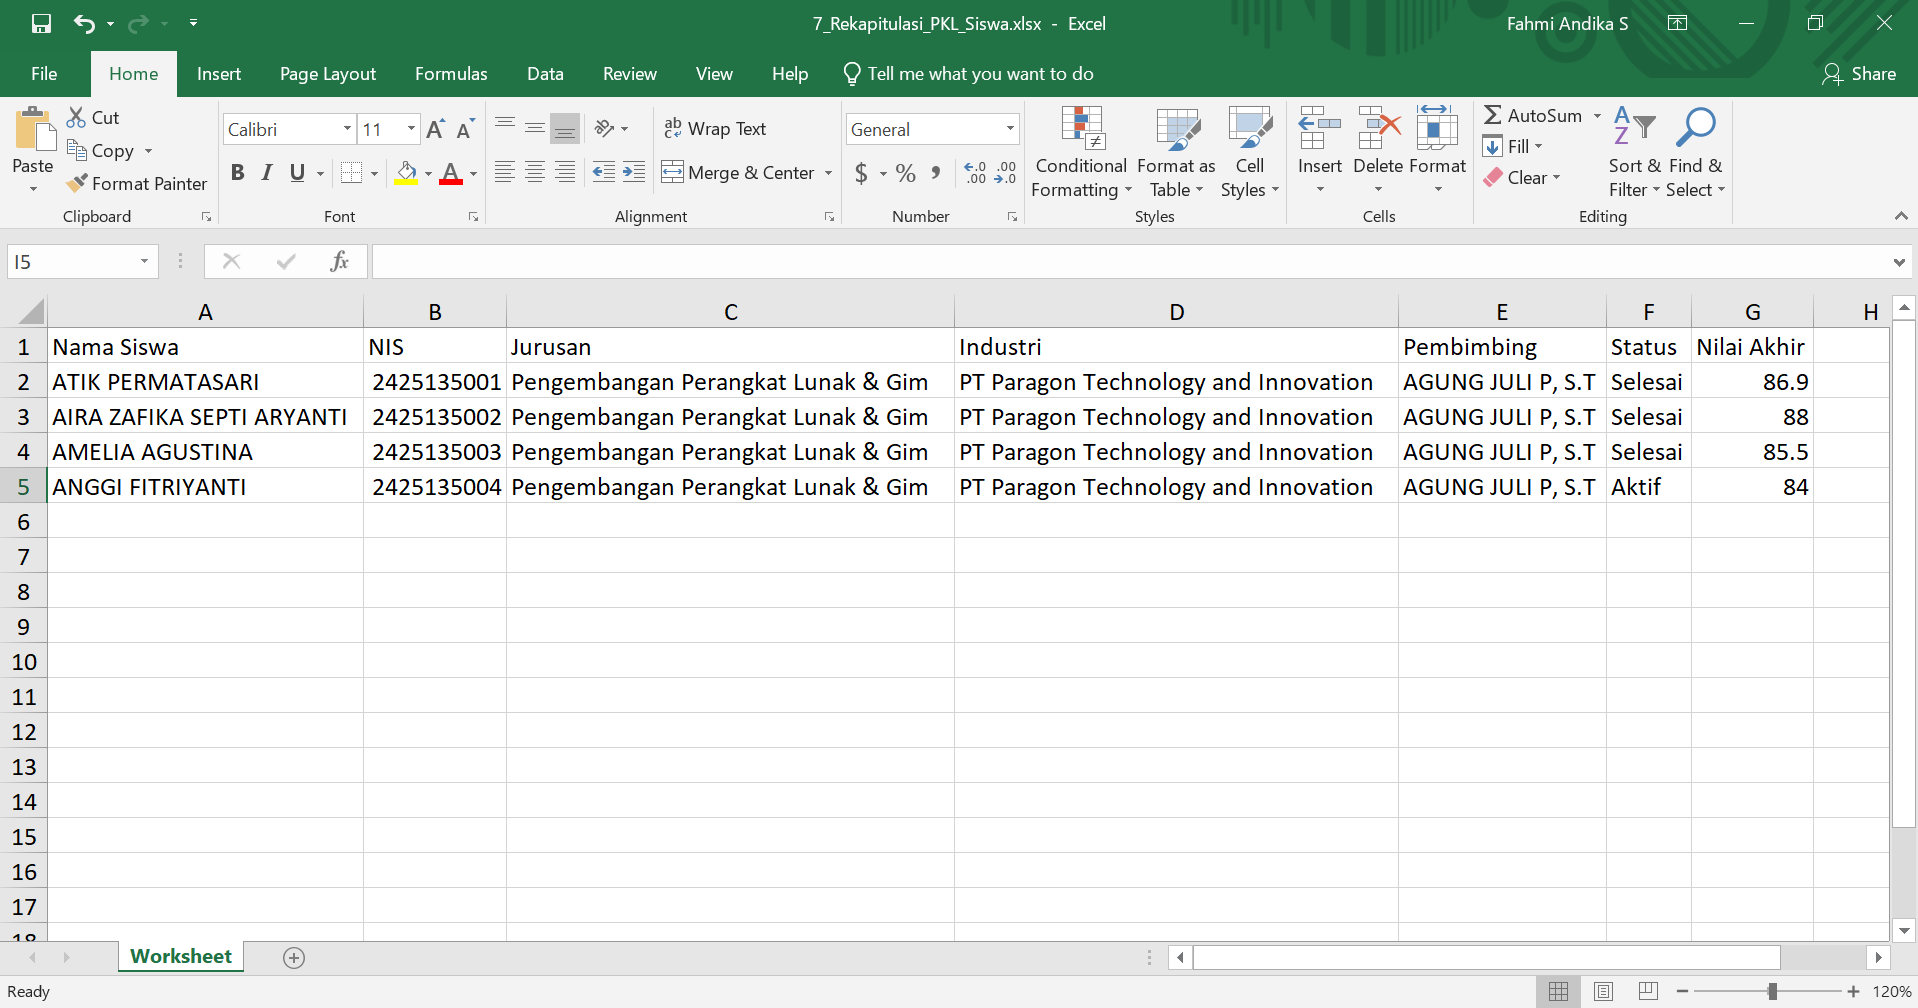
\includegraphics[width=0.94\textwidth,height=0.36\textheight,keepaspectratio]{lampiran/7_Rekapitulasi_PKL_Siswa.png}
\captionof{figure}{Tangkapan layar Rekapitulasi PKL Siswa}\label{fig:lampiran-10}
\end{center}
\clearpage

\begin{center}
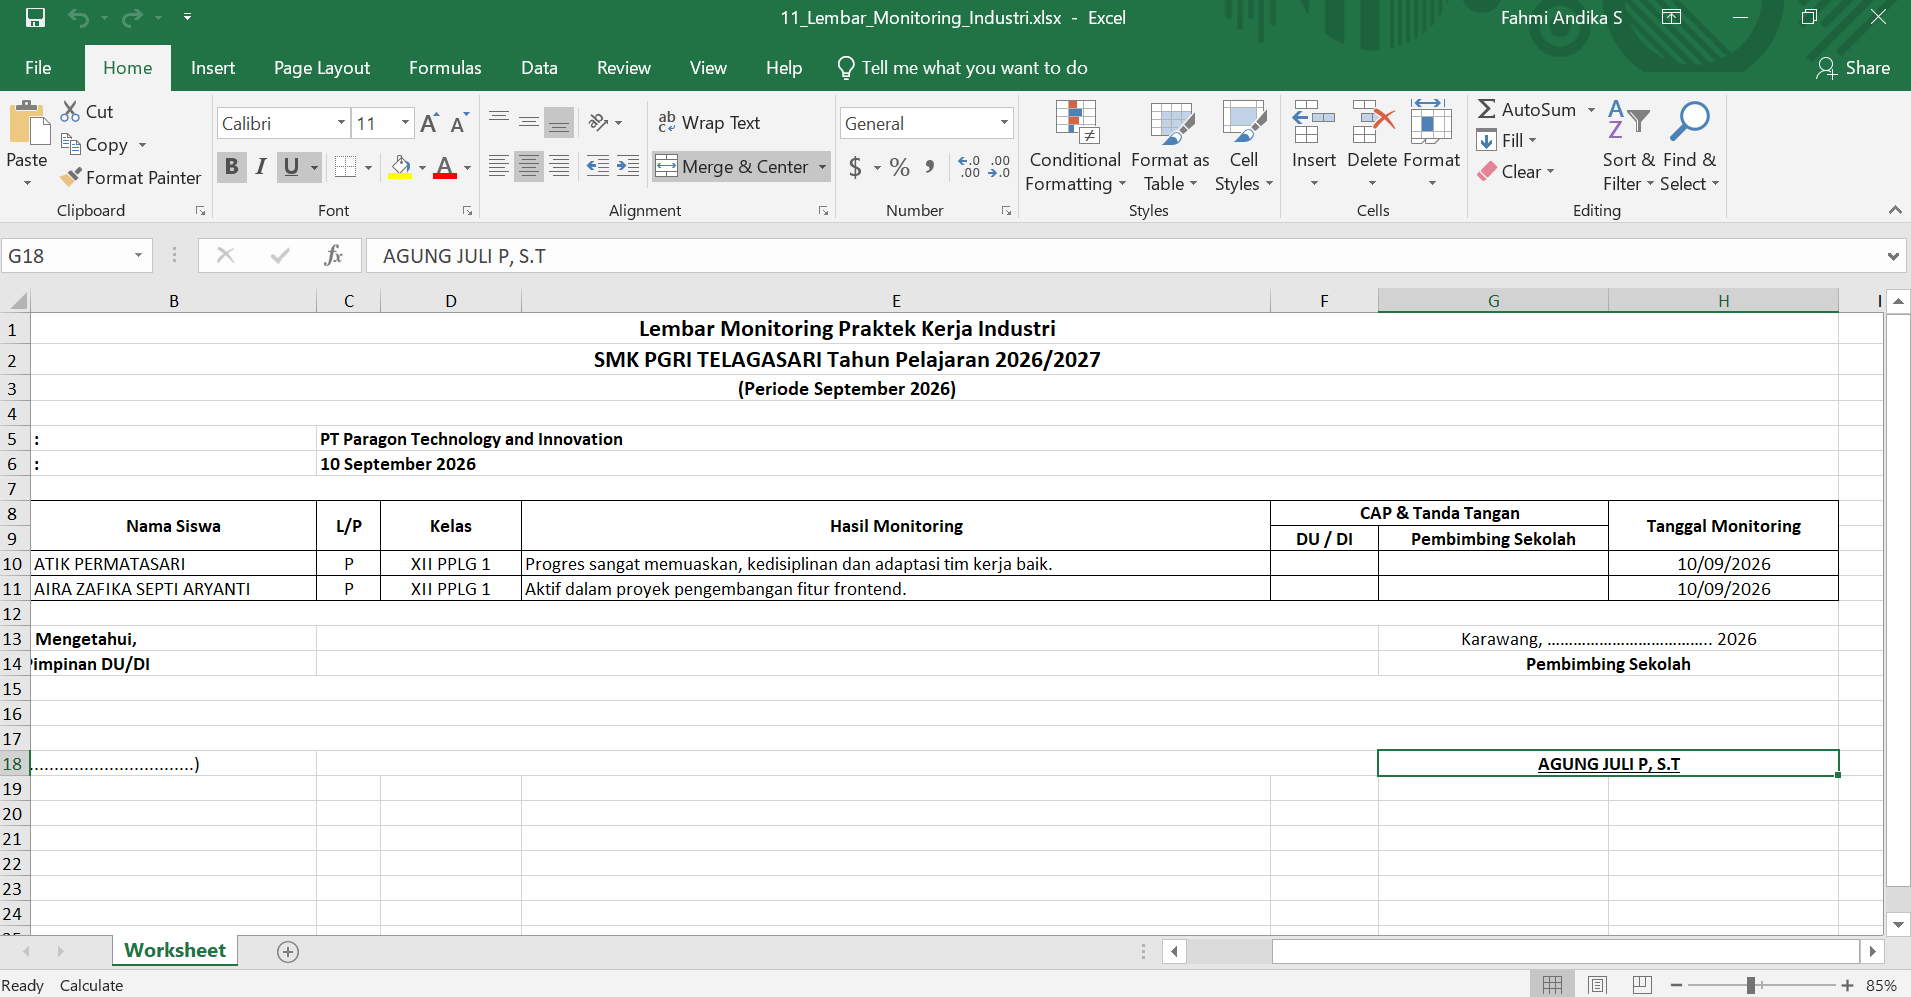
\includegraphics[width=0.94\textwidth,height=0.36\textheight,keepaspectratio]{lampiran/11_Lembar_Monitoring_Industri.png}
\captionof{figure}{Tangkapan layar Lembar Monitoring Industri}\label{fig:lampiran-11}
\end{center}
\medskip
\begin{center}
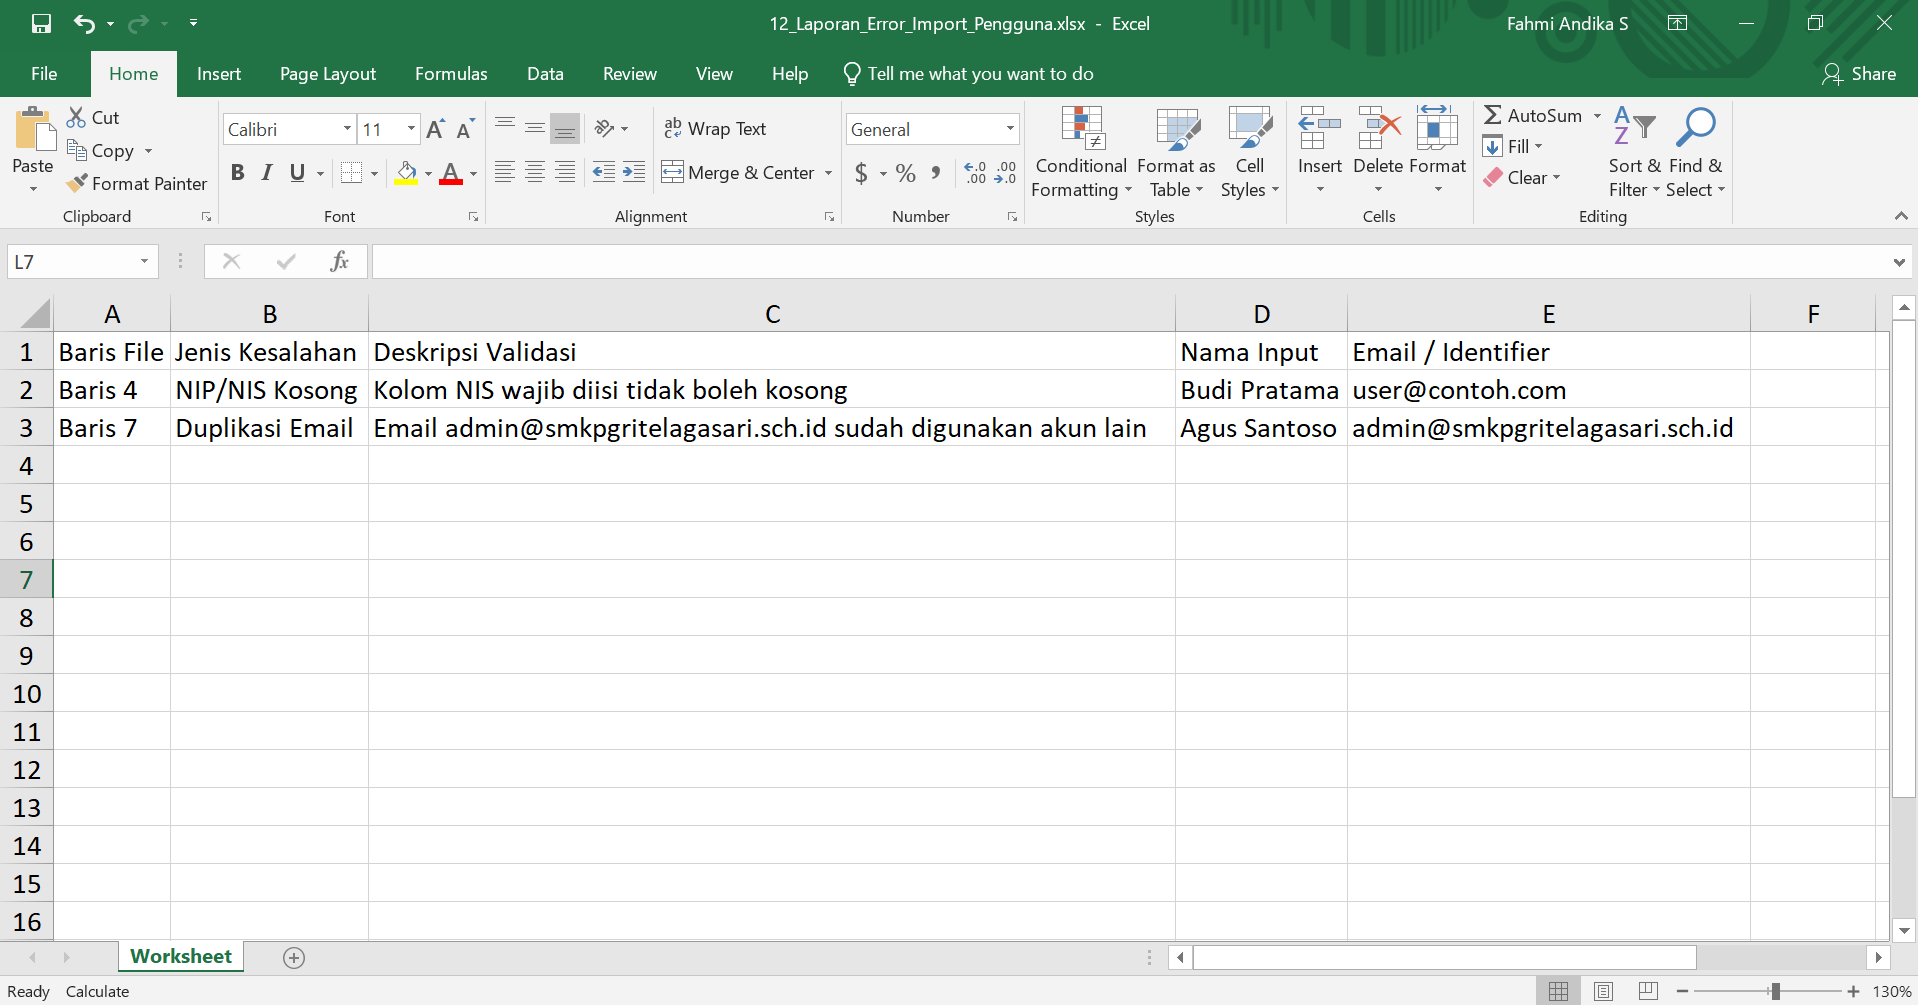
\includegraphics[width=0.94\textwidth,height=0.36\textheight,keepaspectratio]{lampiran/12_Laporan_Error_Import_Pengguna.png}
\captionof{figure}{Tangkapan layar Laporan Kesalahan Impor Pengguna}\label{fig:lampiran-12}
\end{center}
